\chapter{วิธีการดำเนินการวิจัย}
\label{chapter:experiment}

\section{Hybrid Loss}
\subsection{Focal Loss}
สิ่งดลใจในการคิดค้น Focal Loss (FL)~\cite{Lin:2017} คือ Cross Entropy ไม่สามารถควบคุมความสมดุลระหว่างค่าสูญเสียจากกลุ่มข้อมูลส่วนมากและค่าสูญเสียจากกลุ่มข้อมูลส่วนน้อยได้ เพราะข้อมูลจากทั้งสองกลุ่มไม่สมดุลกัน แม้ว่าการใส่ Weighting Factor ($\alpha$) จะสามารถแก้ปัญหานี้ได้ในเบื้องต้น แต่มันก็ไม่สามารถที่จะแยกความแตกต่างระหว่าง ตัวอย่างที่ง่าย (ตัวอย่างที่ให้ค่าสูญเสียน้อย) และ ตัวอย่างที่ยาก (ตัวอย่างที่ให้ค่าสูญเสียมาก) ได้ ซึ่งตัวอย่างที่ง่ายของกลุ่มข้อมูลส่วนมากจะส่วนในการคำนวณค่าสูญเสียรวมมาก ทำให้มีอิทธิพลต่อการคำนวณค่า Gradient มากเช่นเดียวกัน ซึ่งโดยปกติแล้วตัวอย่างที่ยากของกลุ่มข้อมูลส่วนมากจะประกอบไปด้วยข้อมูลที่เป็นประโยชน์ต่อการจัดกลุ่มมากกว่าตัวอย่างที่ง่ายของ
กลุ่มข้อมูลส่วนน้อย~\cite{Zhu:2019} ดังนั้นการเรียนรู้จากตัวอย่างที่ยากของกลุ่มข้อมูลส่วนมากจะมีประสิทธิภาพมากกว่าการเรียนรู้จากตัวอย่างที่ง่ายของกลุ่มข้อมูลส่วนมาก

จากที่กล่าวมาข้างต้นทำให้มีความจำเป็นที่จะต้องลดการมีส่วนร่วมในการคำนวณค่าสูยเสียรวมของตัวอย่างที่ง่าย และให้ความสนใจที่การมีส่วนร่วมในการคำนวณค่าสูยเสียรวมของตัวอย่างที่ยาก ดังนั้น FL ถูกออกแบบมาเพื่อการนี้โดยการเพิ่ม Modulating Factor ($(1 - p_{t})^{\gamma}$) เข้าไปใน Cross Entropy เพื่อที่จะลดน้ำหนักของการเรียนรู้จากตัวอย่างที่ง่าย ที่ซึ่ง Modulating Factor จะช่วยลดการมีส่วนร่วมในการคำนวณค่าสูญเสียรวมจากตัวอย่างที่ง่ายและมุ่งไปที่การเรียนรู้จากตัวอย่างที่ยาก สำหรับการคำนวณค่าสูญเสียและค่าสูญเสียรวมของ FL สามารถคำนวณได้ตามสมการที่~\ref{eq:fl} และ~\ref{eq:tfl} ตามลำดับ

\begin{equation} \label{eq:fl}
FL(p_{t}) = - \alpha_{i}(1 - p_{t})^\gamma \log (p_{t})
\end{equation}

\begin{equation} \label{eq:tfl}
    l_{FL} = \frac{1}{n} \sum_{i = 1}^{n} -\alpha_{i}(1 - p_{t}^{i})^{\gamma}\log (p_{t}^{i})
\end{equation}

สมการด้านบนเป็น FL ในรูปแบบที่เพิ่ม Weighting Factor เข้ามาด้วยเพื่อควบคุมความสมดุลระหว่างค่าสูญเสียจากกลุ่มข้อมูลส่วนมากและค่าสูญเสียจากกลุ่มข้อมูลส่วนน้อย โดยที่ $\gamma$ คือ Focusing Parameter และสำหรับค่าของ $p_{t}$ สามารถถูกระบุได้ดังสมการที่~\ref{eq:p}

\begin{equation} \label{eq:p}
	p_{t} = 
	\begin{cases}
		p & \text{ if } y = 1\\ 
		1 - p & \text{ otherwise, } 
	\end{cases}
\end{equation} 

โดยที่ $p$ คือ ค่าความน่าจะเป็นในการทำนายของโมเดล ดังนั้น $p_{t}^{i}$ คือ ค่า $p_{t}$ ของตัวอย่าง $i$

ในทางปฎิบัติ $\alpha_{i}$ จะมีค่าเท่ากับ $\alpha$ ถ้ากลุ่มข้อมูลของตัวอย่าง $i$ คือ กลุ่มข้อมูลส่วนน้อย และจะมีค่าเท่ากับ $1-\alpha$ ถ้ากลุ่มข้อมูลของตัวอย่าง $i$ คือ กลุ่มข้อมูลส่วนมาก

\subsection{Mean False Error}
Mean False Error (MFE)~\cite{Wang:2016} เป็นฟังก์ชันสูญเสียที่ถูกแก้ไขมาจาก Mean Squared Error (MSE) สิ่งจูงใจในการคิดค้นฟังก์ชันสูญเสียนี้ขึ้นมา คือ MSE ไม่สามารถตรวจจับค่าสูญเสียจากกลุ่มข้อมูลส่วนน้อยได้อย่างมีประสิทธิภาพ พูดง่าย ๆ คือ ค่าสูญเสียรวมที่คำนวณด้วย MSE มันจะมาจากค่าเฉลี่ยของค่าสูญเสียของข้อมูลทั้งหมด โดยสมการคำนวณค่าสูญเสียของ MSE และ สมการคำนวณค่าสูญเสียรวม แสดงดังสมการที่~\ref{eq:mse} และ~\ref{eq:tmse} ตามลำดับ

\begin{equation} \label{eq:mse}
    MSE = \frac{1}{2}(y - d)^{2}
\end{equation}

\begin{equation} \label{eq:tmse}
    l_{MSE} = \frac{1}{n}\sum_{i=1}^{n}\frac{1}{2}(y^{i} - d^{i})^{2}
\end{equation}

จากสมการด้านบน $l$ คือ ค่าสูญเสียรวม, $n$ คือ จำนวนตัวอย่างทั้งหมด, $y^{i}$ ค่ากลุ่มข้อมูลจริงของตัวอย่าง $i$ และ $d^{i}$ คือ ค่าทำนายของโมเดลของตัวอย่าง $i$ โดยที่ $d$ สามารถคำนวณได้จากฟังก์ชัน Logistic ใด ๆ เช่น ฟังก์ชัน Sigmoid ดังสมการที่~\ref{eq:sigmoid} เป็นต้น

\begin{equation} \label{eq:sigmoid}
d =  \frac{\mathrm{1} }{\mathrm{1} + e^{-x} }
\end{equation}

โดยที่ $x$ คือ เอ๊าต์พุตจาก Layer ก่อนหน้า

จากคำนวณค่าสูญเสียรวมด้วย MSE นั้นหมายความว่าค่าสูญเสียจากกลุ่มข้อมูลส่วนมากจะไปกลบค่าสูญเสียจากกลุ่มข้อมูลส่วนน้อย เนื่องจากจำนวนตัวอย่างของกลุ่มข้อมูลส่วนมากนั้นมีมากกว่า เพื่อที่จะแก้ปัญหานี้ MFE ถูกออกแบบให้สามารถคำนวณค่าสูญเสียรวมด้วยการรวมกันระหว่าง ค่าสูญเสียเฉลี่ยของกลุ่มข้อมูลส่วนน้อย กับ ค่าสูญเสียเฉลี่ยของกลุ่มข้อมูลส่วนมาก ตามสมการที่~\ref{eq:mfe} ซึ่ง

\begin{equation} \label{eq:mfe}
    l_{MFE} = \frac{1}{n\_major}\sum_{i=1}^{n\_major}\frac{1}{2}(y^{i} - d^{i})^{2} +\frac{1}{n\_minor}\sum_{i=1}^{n\_minor}\frac{1}{2}(y^{i} - d^{i})^{2}
\end{equation}

โดยที่ $n\_major$ คือ จำนวนตัวอย่างของกลุ่มข้อมูลส่วนมาก และ $n\_minor$ คือ จำนวนตัวอย่างของกลุ่มข้อมูลส่วนน้อย

ผลการทดลองใช้ MFE ในการเรียนรู้ของโมเดลกับชุดข้อมูล CIFAR-100 แสดงให้เห็นว่า MFE สามารถให้ผลการทำนายที่แม่นยำมากกว่า MSE อย่างสิ้นเชิง~\cite{Wang:2016}

\subsection{นิยามของ Hybrid Loss}
คุณสมบัติที่สำคัญของ FL คือ มันสามารถควบความแตกต่างระหว่างตัวอย่างที่ง่ายและตัวอย่างที่ยาก ยิ่งไปกว่านั้นการที่เพิ่ม $\alpha$ เข้าไปในการคำนวณค่าสูญเสียยังช่วยทำให้ความสำคัญของตัวอย่างของกลุ่มข้อมูลส่วนน้อยและส่วนมากมีความสมดุลกัน อย่างไรก็ตามในเมื่อค่าสูญเสียรวมคือค่าเฉลี่ยของค่าสูญเสียของข้อมูลทั้งหมด มันก็ยังมีโอกาสที่ค่าสูญเสียจากกลุ่มข้อมูลส่วนมากจะไปกลบค่าสูญเสียจากกลุ่มข้อมูลส่วนน้อย ถ้าเราแก้ปัญหาด้วยการกำหนดค่า $\alpha$ ให้มีค่าที่มาก ก็อาจจะช่วยแก้ปัญหานี้ได้ในเบื้องต้น ผลการทดลองใน~\cite{Lin:2017} ได้แสดงให้เห็นว่าการที่ $\alpha$ มีค่าที่มากก็ไม่ทำให้ประสทธิภาพของโมเดลดีไปกว่าค่าที่น้อยกว่าเลย ดังนั้นการเพิ่ม $\alpha$ เข้าไปในการคำนวณค่าสูญเสียอาจจะไม่เพียงพอในการแก้ปัญหานี้

เพื่อที่จะควบคุมค่าสูญเสียจากกลุ่มข้อมูลส่วนมากและกลุ่มข้อมูลส่วนน้อยให้มีความสมดุลกันอย่างสิ้นเชิง
ในงานวิจัยนี้จึงได้เสนอที่จะนำรูปแบบการคำนวณค่าสูญเสียรวมของ MFE มาประยุกต์ใช้ร่วมกับการคำนวณค่าสูญเสียของ FL กล่าวคือ การคำนวณค่าสูญเสียของแต่ละตัวอย่างยังคงเหมือนเดิมตามการคำนวณด้วย FL แต่ในการคำนวณค่าสูญเสียรวมจะเป็นการนำค่าสูญเสียเฉลี่ยของกลุ่มข้อมูลส่วนมากและค่าสูญเสียเฉลี่ยของกลุ่มข้อมูลส่วนน้อยมาบวกกัน ดังสมการที่~\ref{eq:hybird1}

\begin{equation} \label{eq:hybird1}
    l_{Hybrid} = \frac{1}{n\_major} \sum_{i = 1}^{n\_major} -\alpha_{i}(1 - p_{t}^{i})^{\gamma}\log (p_{t}^{i}) + \frac{1}{n\_minor} \sum_{i = 1}^{n\_minor} -\alpha_{i}(1 - p_{t}^{i})^{\gamma}\log (p_{t}^{i})
\end{equation}

\subsection{การหาอนุพันธ์}

\subsubsection{อนุพันธ์ของ FL}
กำหนดให้มี $x$ และ $y$ โดยที่ $y$ คือ ค่ากลุ่มข้อมูลจริง สมมติให้

\begin{equation}
	p = \sigma (x) = \frac{1}{1 + e^{-x}}
\end{equation}

ดังนั้น

\begin{equation}
	p_{t} = \frac{1}{1 + e^{xy}}
\end{equation}

เมื่อหาอนุพันธ์ของ $p_{t}$ เทียบกับ $x$ จะได้

\begin{equation}
\frac{dp_{t}}{dx} = y(1 - p_{t})p_{t}
\end{equation}

กำหนดให้

\begin{equation}
    l_{FL} = \frac{1}{n} \sum_{i = 1}^{n} - (1 - p_{t}^{i})^{\gamma}\log (p_{t}^{i})
\end{equation}

โดยที่ $\gamma$ เป็นค่าคงที่ เมื่อหาอนุพันธ์ของ $l_{FL}$ เทียบกับ $x$จะได้

\begin{equation}
\begin{split}
\frac{dl_{FL}}{dx} & = \frac{1}{n} \sum_{i = 1}^{n} (\frac{dl_{FL}}{dp_{t}^{i}} * \frac{dp_{t}^{i}}{dx^{i}}) \\
& =\frac{1}{n} \sum_{i = 1}^{n} [\gamma (1 - p_{t}^{i})^{\gamma - 1} \log (p_{t}^{i}) + \frac{(1 - p_{t}^{i})^{\gamma}}{p_{t}^{i}}] * [y^{i}(1 - p_{t}^{i})p_{t}^{i}]  \\
& = \frac{1}{n} \sum_{i = 1}^{n} y^{i} (1 - p_{t}^{i})^{\gamma} (\gamma p_{t}^{i} \log (p_{t}^{i}) + p_{t}^{i} - 1)
\end{split}
\end{equation}

\subsubsection{อนุพันธ์ของ MFE}
กำหนดให้

\begin{equation}
MSE_{major} = \frac{1}{n\_major}\sum_{i=1}^{n\_major}\frac{1}{2}(y^{i} - d^{i})^{2}
\end{equation}

\begin{equation}
MSE_{minor} = \frac{1}{n\_minor}\sum_{i=1}^{n\_minor}\frac{1}{2}(y^{i} - d^{i})^{2}
\end{equation}

ดังนั้น

\begin{equation}
    l_{MFE} = MSE_{major} + MSE_{minor}
\end{equation}

เมื่อหาอนุพันธ์ของ $l_{MFE}$ เทียบกับ $x$ จะได้

\begin{equation}
\frac{dl_{MFE}}{dx} = \frac{dMSE_{major}}{dx} + \frac{dMSE_{minor}}{dx}
\end{equation}

โดยที่

\begin{equation} \label{eq:fpe_derivative}
\frac{dMSE_{major}}{dx} = - \frac{1}{n\_major} \sum_{i=1}^{n\_major} (y^{i} - d^{i}) d^{i} (1 - d^{i})
\end{equation}

\begin{equation} \label{eq:fne_derivative}
\frac{dMSE_{minor}}{dx} = - \frac{1}{n\_minor} \sum_{i=1}^{n\_minor} (y^{i} - d^{i}) d^{i} (1 - d^{i})
\end{equation}

เราจะใช้อนุพันธ์ที่ต่างกันสำหรับตัวอย่างของแต่ละกลุ่มข้อมูล กล่าวคือ ถ้าเป็นตัวอย่างของกลุ่มข้อมูลส่วนมาก สมการที่~\ref{eq:fpe_derivative} จะถูกใช้ และสมการที่~\ref{eq:fne_derivative} จะถูกใช้เมื่อตัวย่างเป็นของกลุ่มข้อมูลส่วนน้อย



\subsubsection{อนุพันธ์ของ Hybrid Loss}
กำหนดให้

\begin{equation}
    FL_{major} = \frac{1}{n\_major} \sum_{i = 1}^{n\_major} - (1 - p_{t}^{i})^{\gamma}\log (p_{t}^{i})
\end{equation}

\begin{equation}
    FL_{minor} = \frac{1}{n\_minor} \sum_{i = 1}^{n\_minor} - (1 - p_{t}^{i})^{\gamma}\log (p_{t}^{i})
\end{equation}

ดังนั้น

\begin{equation}
    l_{Hybrid} = FL_{major} + FL_{minor}
\end{equation}

เมื่อหาอนุพันธ์ของ $l_{Hybrid}$ เทียบกับ x จะได้

\begin{equation}
\frac{dl_{Hybrid}}{dx} = \frac{dFL_{major}}{dx} + \frac{dFL_{minor}}{dx}
\end{equation}

โดยที่

\begin{equation} \label{fl_major_derivative}
\frac{dFL_{major}}{dx} = \frac{1}{n\_major} \sum_{i = 1}^{n\_major} y^{i} (1 - p_{t}^{i})^{\gamma} (\gamma p_{t}^{i} \log (p_{t}^{i}) + p_{t}^{i} - 1)
\end{equation}

\begin{equation} \label{fl_minor_derivative}
\frac{dFL_{minor}}{dx} = \frac{1}{n\_minor} \sum_{i = 1}^{n\_minor} y^{i} (1 - p_{t}^{i})^{\gamma} (\gamma p_{t}^{i} \log (p_{t}^{i}) + p_{t}^{i} - 1)
\end{equation}

เช่นเดียวกับการใช้อนุพันธ์ของ MFE ก็คือ เราจะใช้สมการที่~\ref{fl_major_derivative} ถ้าตัวอย่างเป็นของกลุ่มข้อมูลส่วนมาก และจะใช้สมการที่~\ref{fl_minor_derivative} ถ้าตัวอย่างเป็นของกลุ่มข้อมูลส่วนน้อย

\section{Metrics สำหรับการประเมินประสิทธิภาพของโมเดล}
\subsection{F1-Score}
F1-Score เป็นค่าเฉลี่ยของ Precision และ Recall ที่ซึ่งเราสามารถพิจารณาประสิทธิภาพของแบบจำลองด้วย F1-Score แทนการพิจารณาด้วย Precision หรือ Recall โดย F1-Score สามารถคำนวณได้จากสมการที่ \ref{eq:f1-score}

\begin{equation}
  F1 = 2 * \left ( \frac{precision * recall}{precision + recall} \right )
  \label{eq:f1-score}
\end{equation}

โดยที่ Precision และ Recall สามารถคำนวณได้จากสมการที่ \ref{eq:precision} และ \ref{eq:recall} ตามลำดับ

\begin{equation}
  precision = \frac{TP}{TP + FP}
  \label{eq:precision}
\end{equation}

\begin{equation}
  recall = \frac{TP}{TP + FN}
  \label{eq:recall}
\end{equation}

โดยที่

\begin{itemize}
  \item True Positive (TP) คือ จำนวนตัวอย่างที่แบบจำลองตรวจจับได้ว่าเป็น Positive Class และตัวอย่างเหล่านั้นเป็น Positive Class
  \item True Negative (TN) คือ จำนวนตัวอย่างที่แบบจำลองตรวจจับได้ว่าเป็น Negative Class และตัวอย่างเหล่านั้นเป็น Negative Class
  \item False Positive (FP) คือ จำนวนตัวอย่างที่แบบจำลองตรวจจับได้ว่าเป็น Positive Class แต่ตัวอย่างเหล่านั้นเป็น Negative Class
  \item False Negative (FN) คือ จำนวนตัวอย่างที่แบบจำลองตรวจจับได้ว่าเป็น Negative Class แต่ตัวอย่างเหล่านั้นเป็น Positive Class
\end{itemize}

\subsection{Receiver Operating Characteristic Curve (ROC Curve)}
ROC Curve เป็นกราฟความสัมพันธ์ระหว่าง True Positive Rate (TPR) และ False Positive Rate (FPR) โดย TPR หรือ Recall คือ 
ความน่าจะเป็นที่แบบจำลองสามารถตรวจจับ Positive Class จากจำนวน Positive Class ทั้งหมด และ FPR คือ 
ความน่าจะเป็นที่แบบจำลองจะตรวจจับ Positive Class จากจำนวน Negative Class ทั้งหมด ทั้ง TPR และ FPR สามารถคำนวณได้จากสมการที่ \ref{eq:tpr} และ \ref{eq:fpr} ตามลำดับ

\begin{equation}
  TPR = recall = \frac{TP}{TP + FN}
  \label{eq:tpr}
\end{equation}

\begin{equation}
  FPR = \frac{FP}{FP + TN}
  \label{eq:fpr}
\end{equation}

\subsection{Area Under the ROC Curve (AUC)}
AUC คือความน่าจะเป็นที่แบบจำลองจะระบุตัวอย่างของ Positive Class ว่าเป็น Positive Class และตัวอย่างของ Negative Class ว่าเป็น Negative Class 
โดยถ้าค่า AUC เข้าใกล้ 1 นั้นหมายความว่าแบบจำลองมีความสามารถในการแยก Positive Class ออกจาก Negative Class ได้เป็นอย่างดี 
ในทางเทคนิค AUC ก็คือพื้นที่ใต้กราฟของ ROC Curve โดยความสัมพันธ์กันระหว่างค่า AUC และ ROC Curve ถูกแสดงดังรูปที่ \ref{fig:roc}

\begin{figure}[h]
  \centering
  \subfigure[]{
      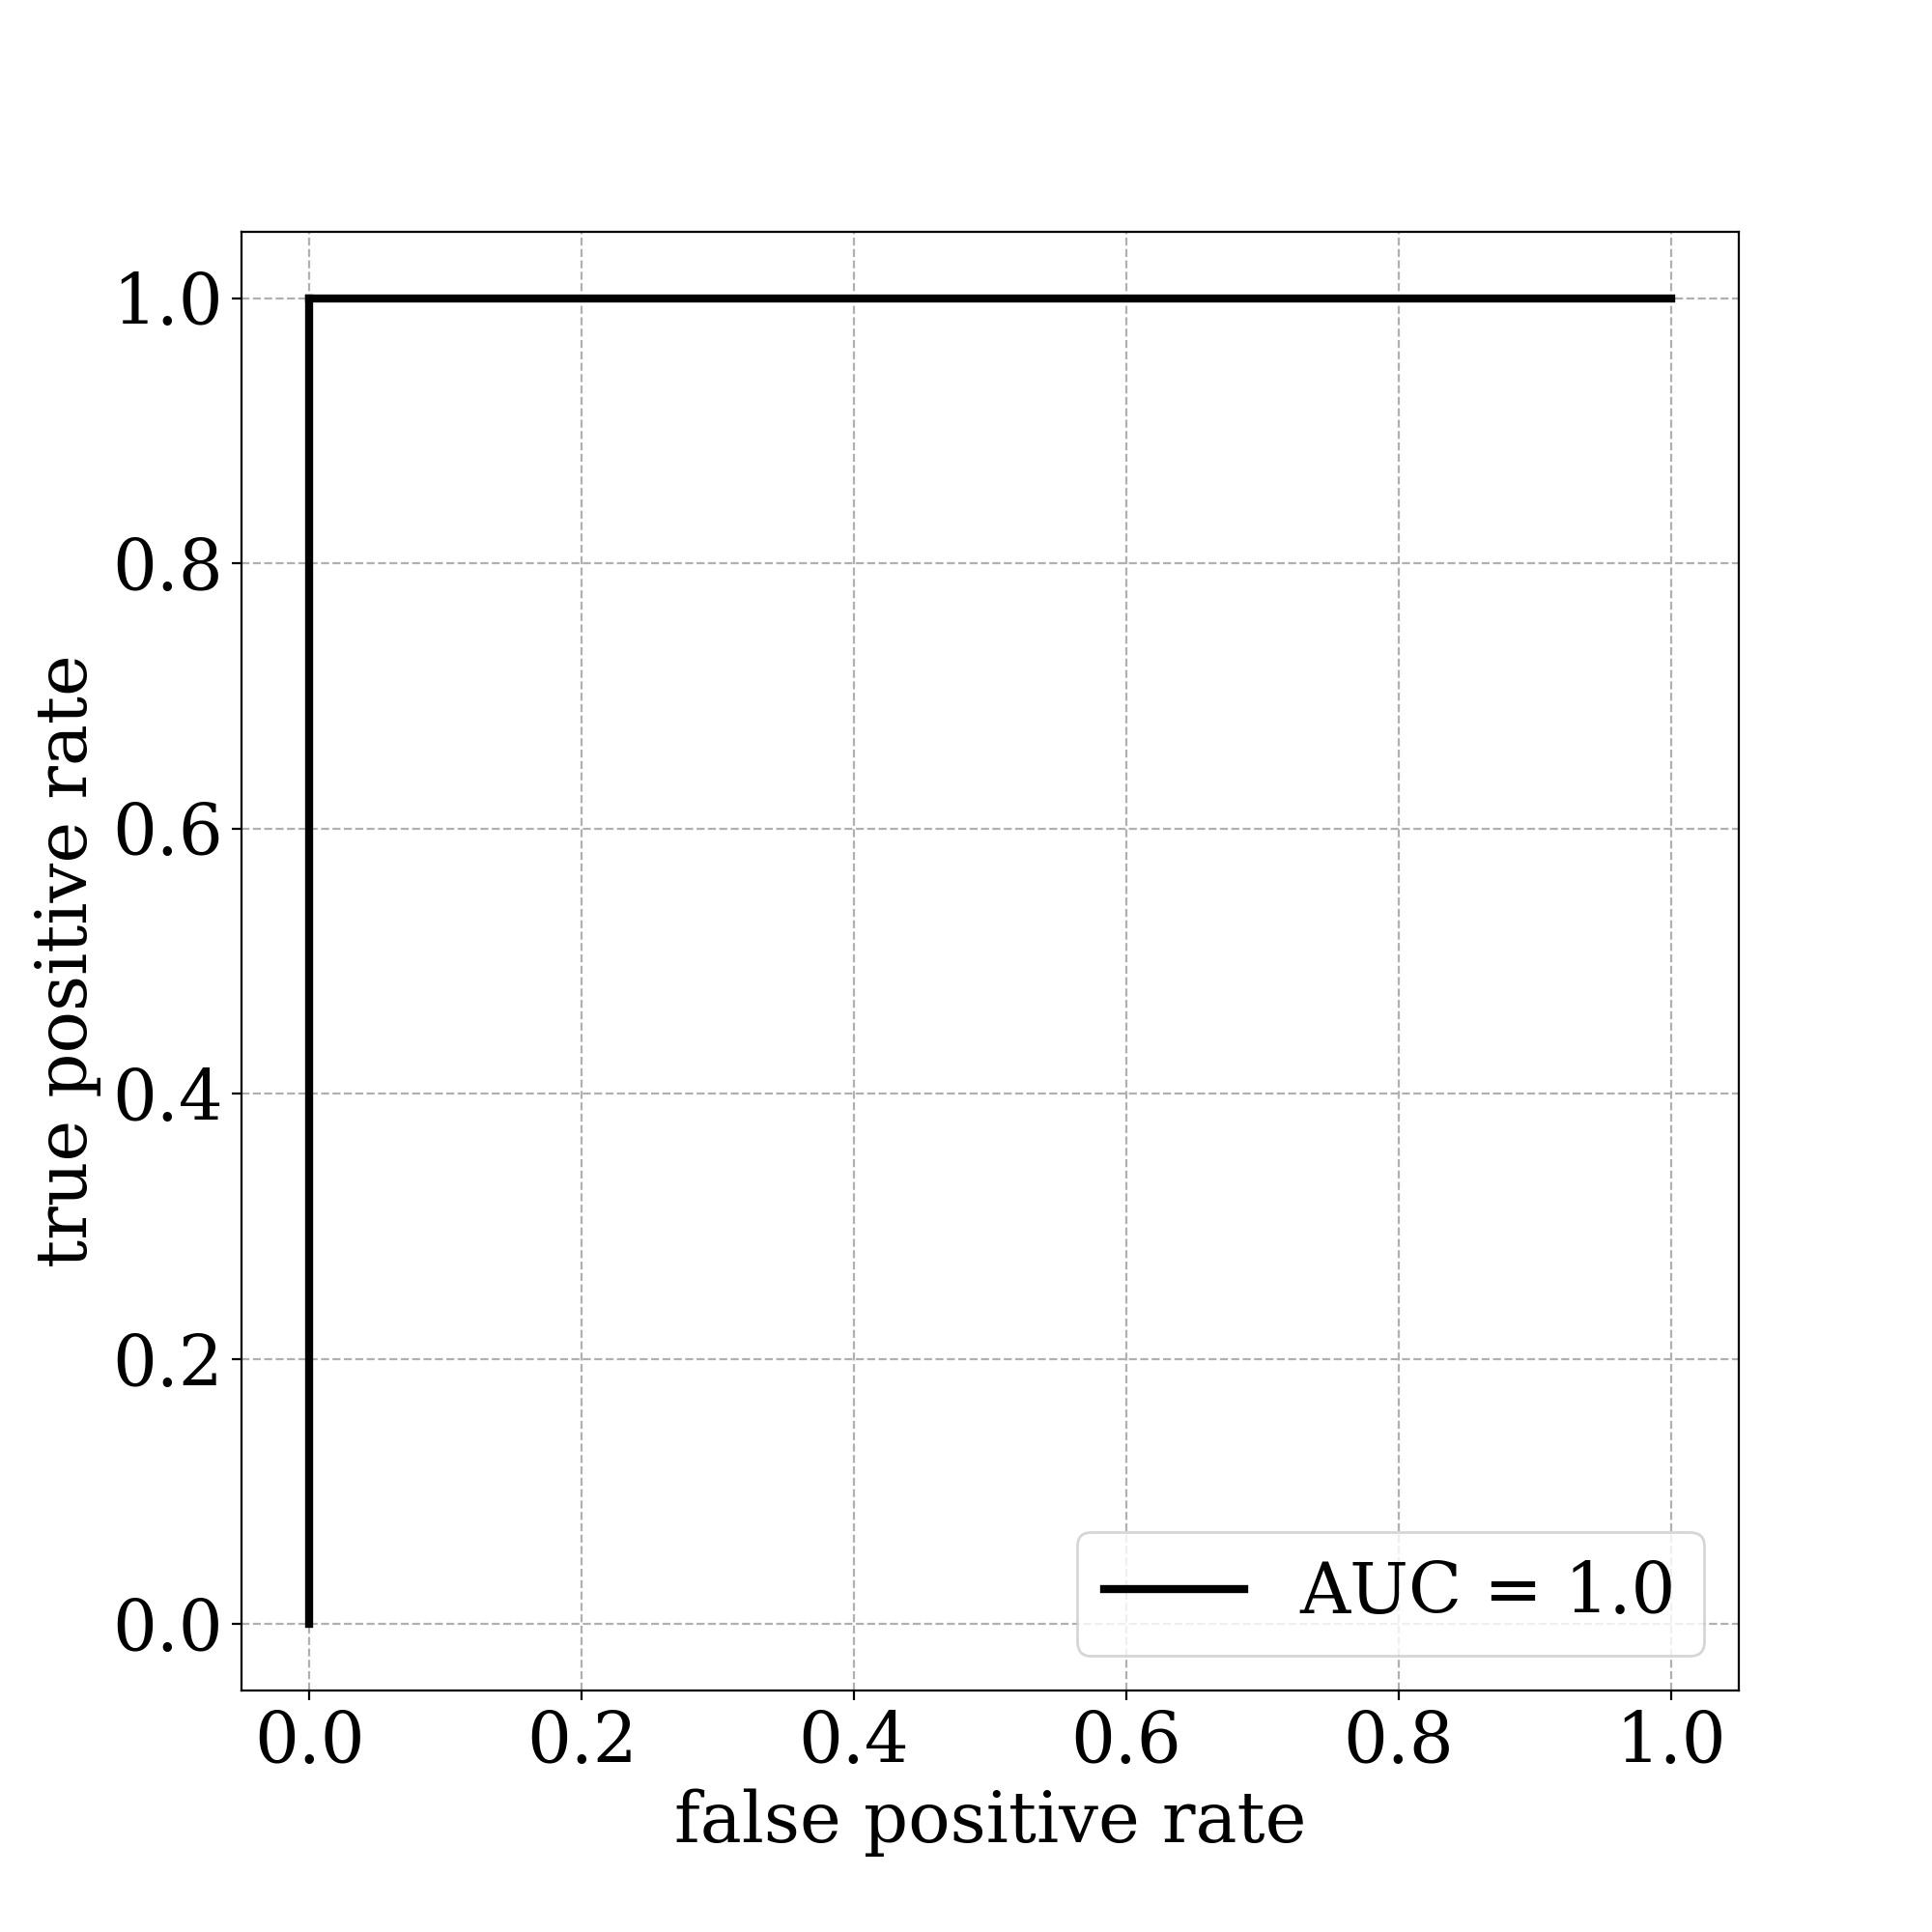
\includegraphics[width=0.45\columnwidth]{roc-1.png}
      \label{fig:roc:1}
  }
  \subfigure[]{
      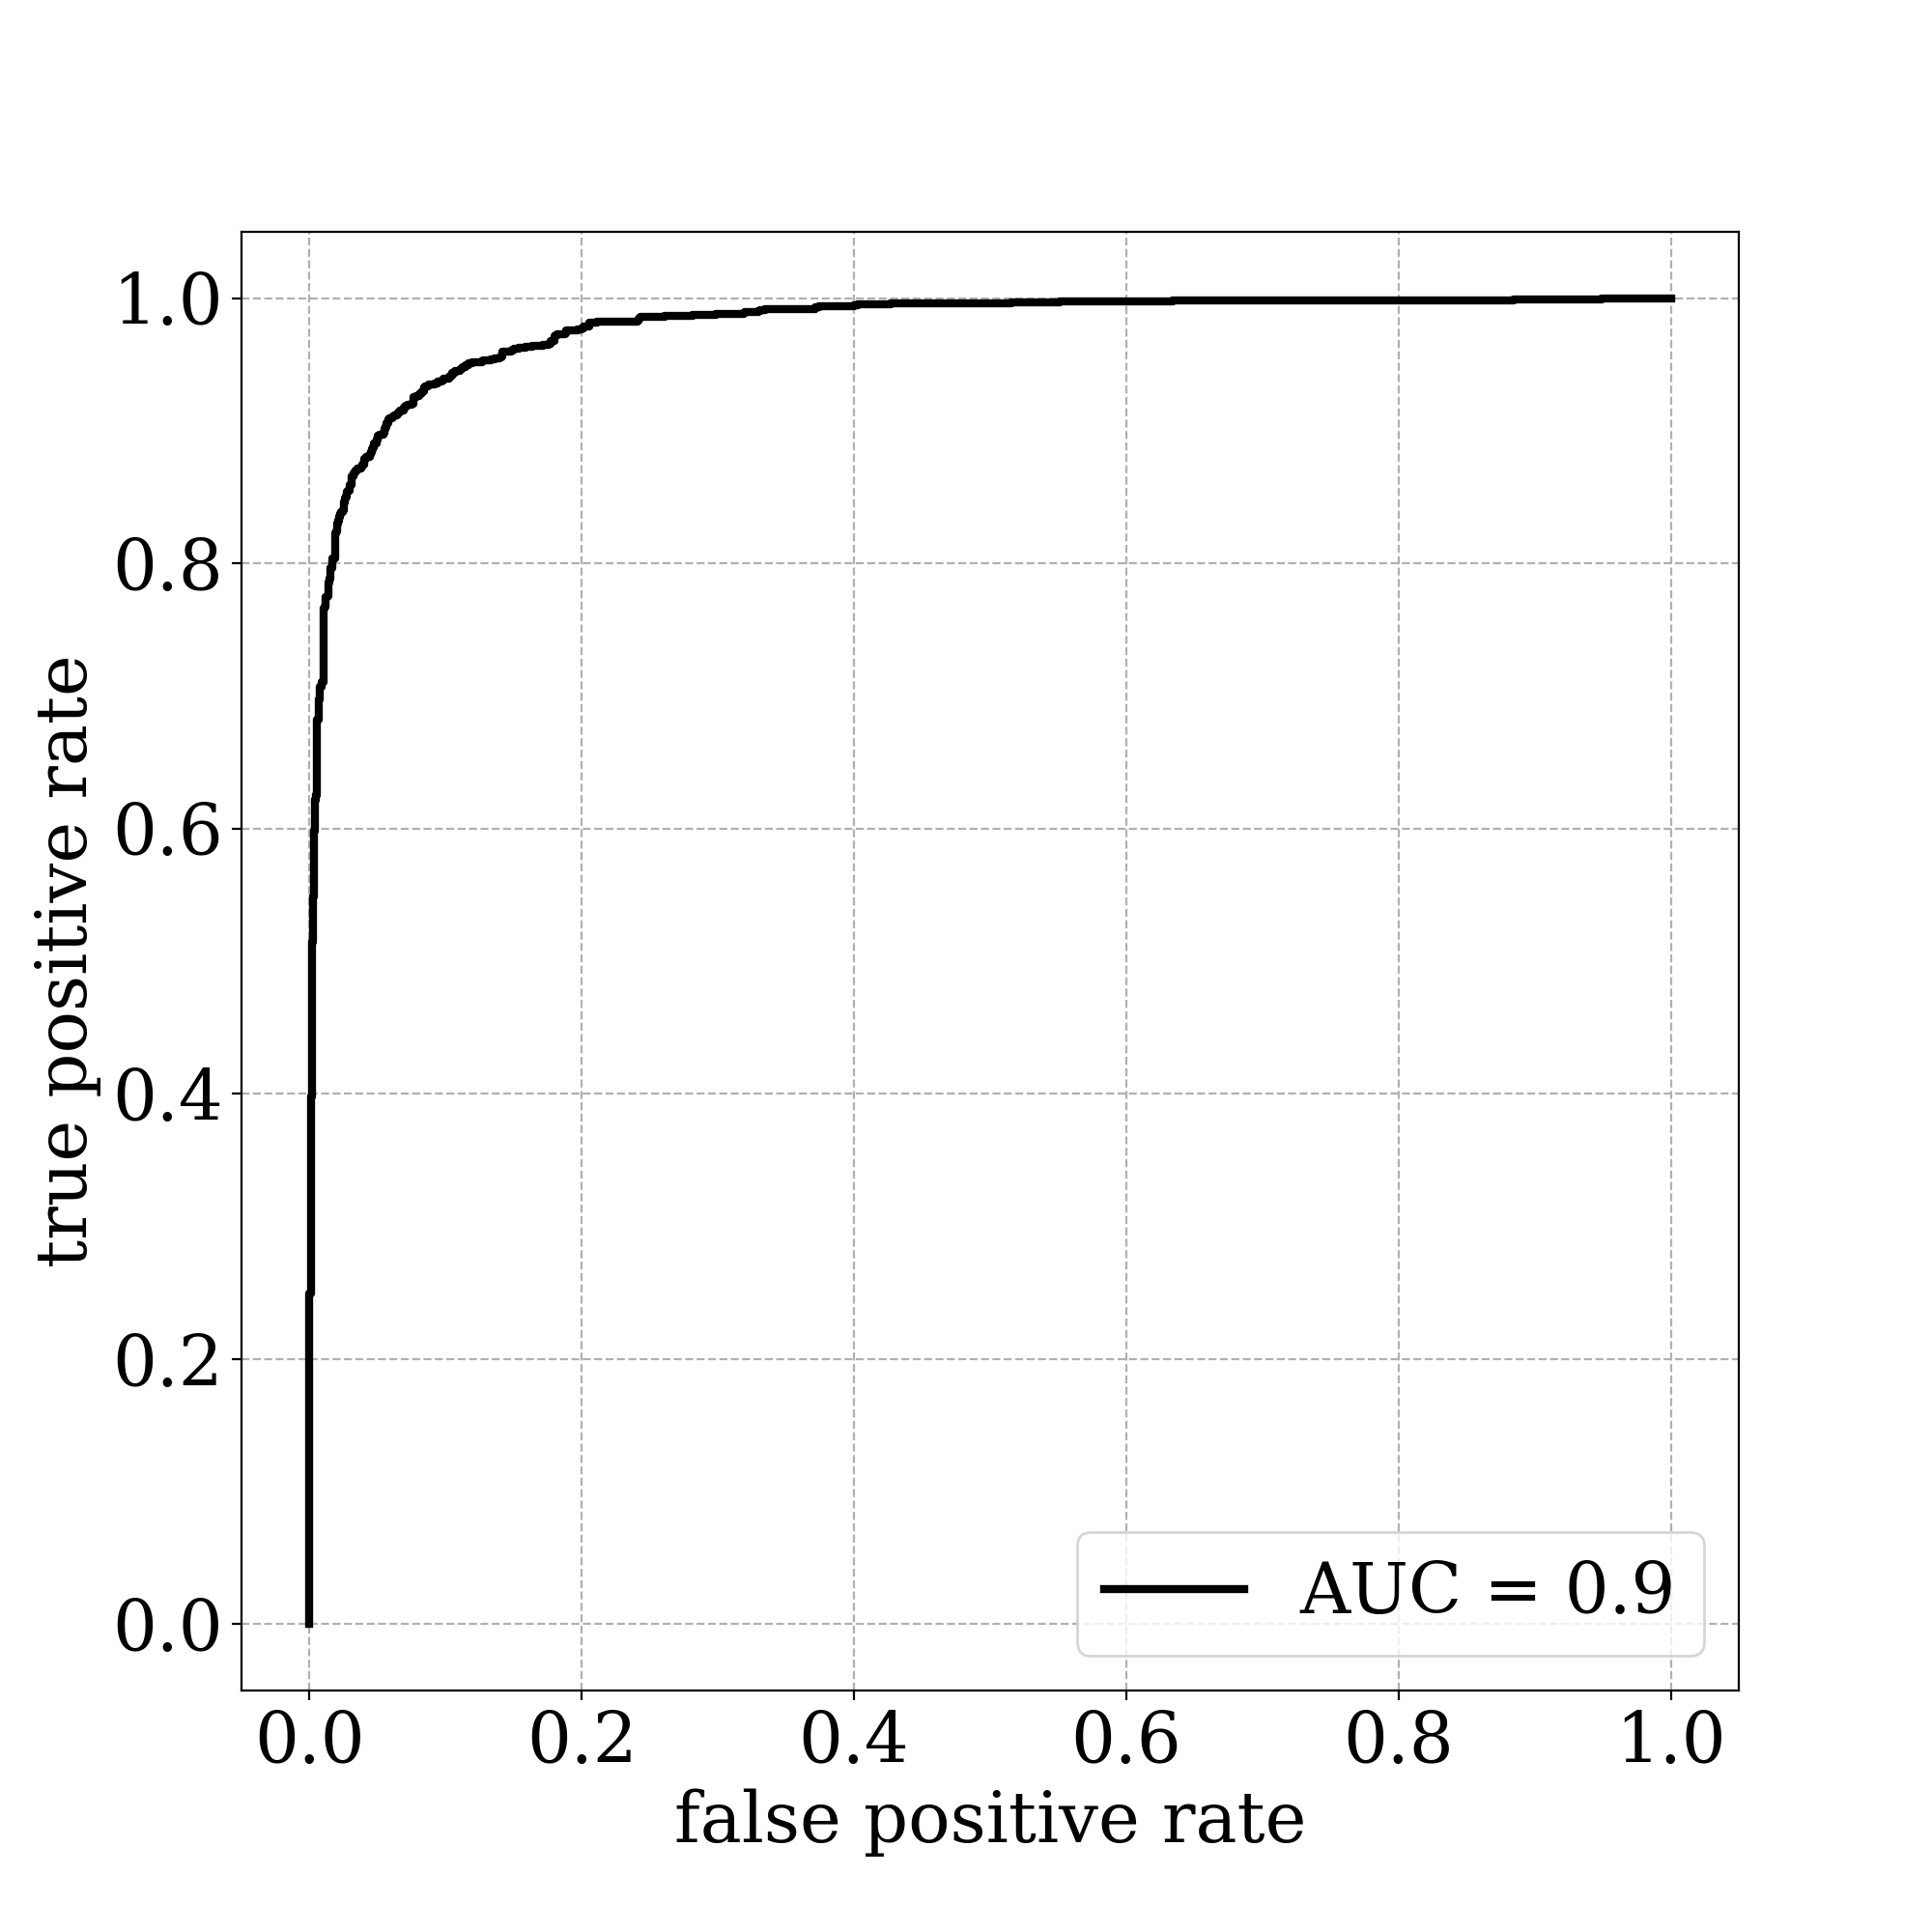
\includegraphics[width=0.45\columnwidth]{roc-2.png}
      \label{fig:roc:3}
  }
  \subfigure[]{
    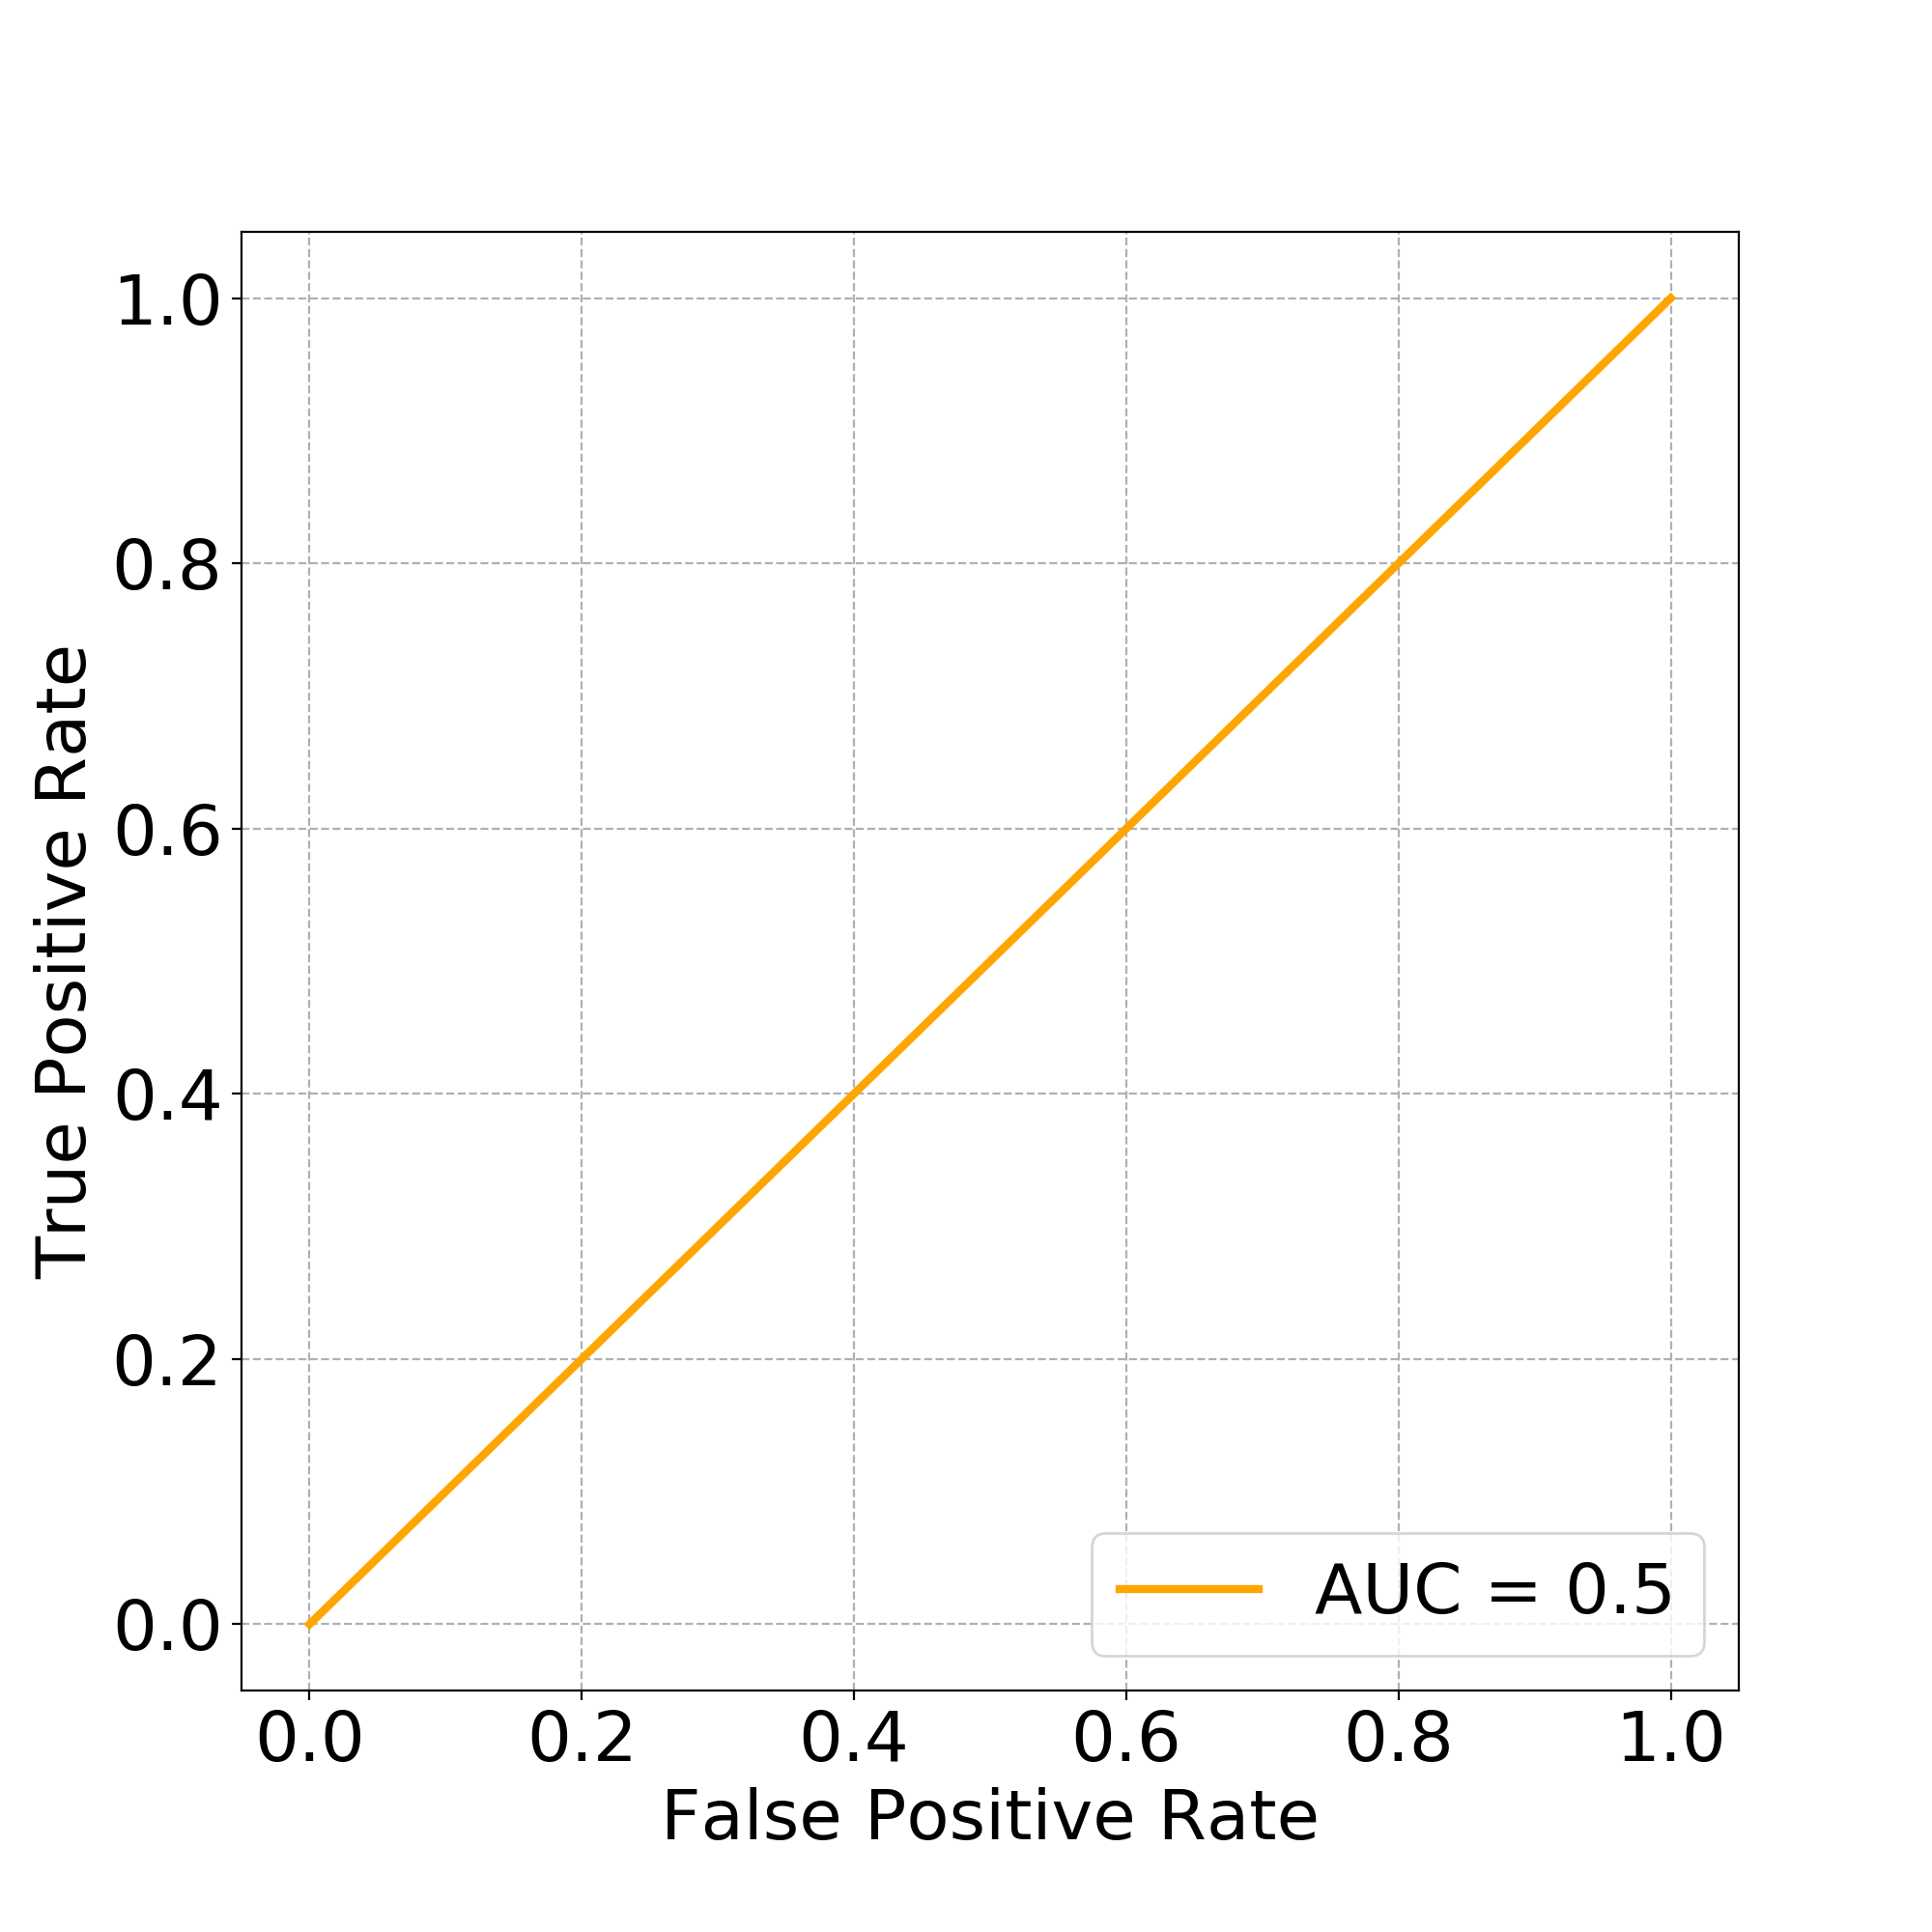
\includegraphics[width=0.45\columnwidth]{roc-3.png}
    \label{fig:roc:3}
  }
  \subfigure[]{
    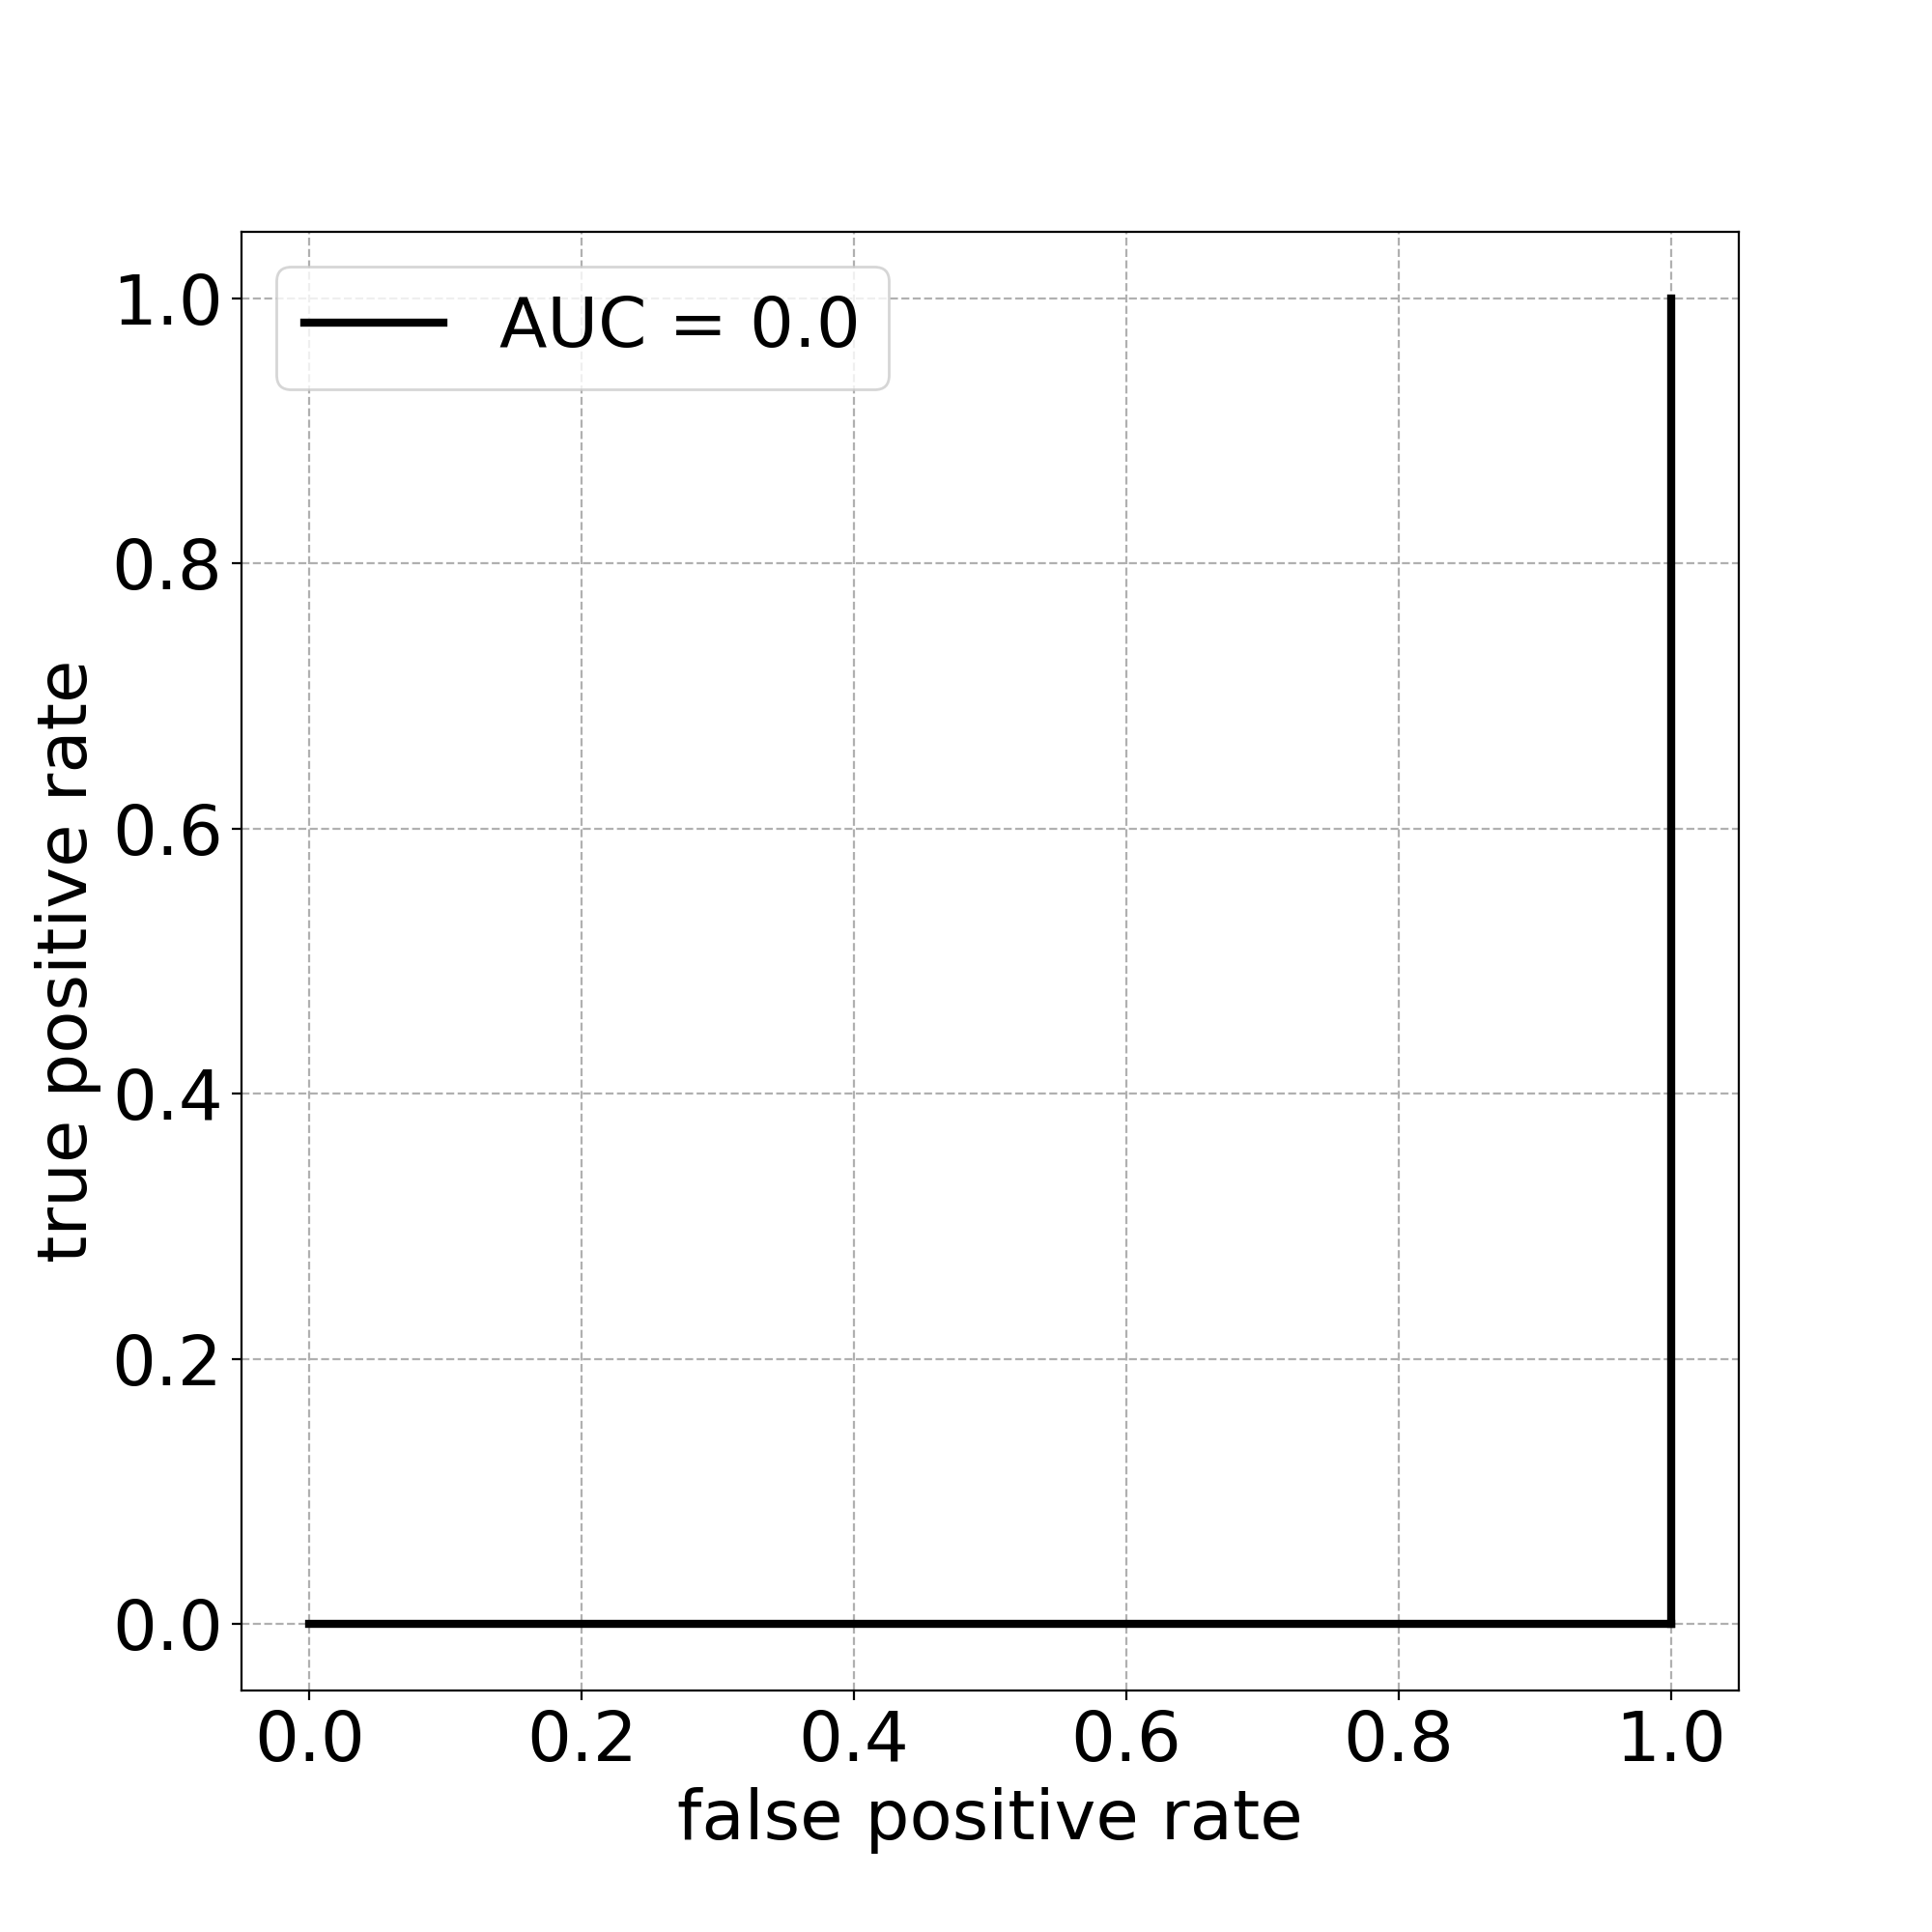
\includegraphics[width=0.45\columnwidth]{roc-4.png}
    \label{fig:roc:3}
  }
  \caption{ตัวอย่างกราฟ ROC Curve แบบต่าง ๆ}
  \label{fig:roc}
\end{figure}
\FloatBarrier
